\chapter{Обзор предметной области}
\label{chap:preliminaries}

\section{Используемые веб-сервисы}
\subsection{Твиттер}
``Твиттер'' является популярной социальной сетью, появившейся в 2006 году, и набравшей с тех пор более 140 миллионов активных пользователей. Основой сервиса являются публикуемые пользователями короткие сообщения, длина которых ограничена 140 символами.

Стоит отметить, что ``Твиттер'' предоставляет прикладной программный интерфейс (API) для доступа к своим данным\footnote{https://dev.twitter.com/docs/api}. Благодаря этому было создано множество библиотек для работы с данными из ``Твиттера'' на различных языках программирования.

В силу популярности сервиса, актуальности анализа его данных, а также удобства работы с ним с точки зрения создания программного обеспечения этот сервис был выбран в качестве источника данных.

\subsection{Википедия}
``Википедия'' представляет из себя свободную общедоступную энциклопедию. Главной особенностью Википедии является то, что каждый её участник может создавать, удалять и редактировать содержимое статей. Благодаря этой особенности англоязычная ``Википедия'' включает в себя порядка 4 миллионов статей (на момент мая 2012 года), а, к примеру, русскоязычная --- 800 тысяч статей\footnote{http://www.wikipedia.org/}.

Структурированность и энциклопедическая природа данных в ``Википедии'' позволяет использовать её при обработке естественных языков, к примеру, в задачах классификации и кластеризации. Данная идея не нова и существует множество исследований на данную тему. К примеру, в работе \cite{Genc:2011:DCC:2021773.2021833} сделана попытка разбить записи из ``Твиттера'' на кластеры с помощью ``Википедии''.

\section{Классификация}
\subsection{Формальное определение}
Классификацией называется задача машинного обучения с учителем. Целью классификации является разделение некоторого множества объектов на конечное, заранее известное, число классов. Для конечного подмножества объектов, называемого обучающей выборкой, класс известен заранее.

Формально, пусть $X$ --- множество описаний объектов, $Y$ --- множество номеров (или наименований) классов. Существует неизвестная ``целевая зависимость'' --- отображение $y^{*}\colon X\to Y$, значения которой известны только на объектах конечной обучающей выборки $X^m = \{(x_1,y_1),\dots,(x_m,y_m)\}$. Требуется построить алгоритм $a\colon X\to Y$, аппроксимирующий целевую зависимость\cite{wiki:ru-classification}.

Большинство алгоритмов классификации для своей работы требуют описания классифицируемых объектов в виде набора некоторых признаков или характеристик. Эти признаки бывают бинарные, номинальные, порядковые и количественные. К примеру, для текста такими признаками могут быть: ``наличие местоимений в тексте'', ``наличие сочетания 'ия' в тексте'', ``средняя длина слова меньше 5'', и т.д.

\subsection{Алгоритмы}
Существует множество подходов для реализации алгоритмов классификации. Стоит выделить такие направления, как байесовские классификаторы, нейронные сети, линейные разделители, деревья решений. Далее более подробно рассматриваются алгоритмы, используемые в данной работе.

\subsubsection{Наивный байесовский классификатор}
Наивный байесовский классификатор (Naive Bayes classifier) основан на использовании теоремы Байеса\footnote{http://ru.wikipedia.org/wiki/Теорема\_Байеса} и предполагает независимость признаков объектов.

Пусть у нас есть объект $D \in X$, имеющий признаки $\{x_1,\dots,x_n\}$, а также класс $C \in Y$. Умея оценивать $\Prob(C \vert D)\,$ мы бы могли построить классификатор по следующему правилу: $\mathrm{classify}(D) = \mathop{\mathrm{argmax}}_C \ \Prob(C \vert D)$.

Оценим $\Prob(C \vert D)$ по теореме Байеса: \begin{gather}
\Prob(C \vert D) = \Prob(C \vert x_1,\dots,x_n) = \frac{\Prob(C) \ \Prob(x_1,\dots,x_n\vert C)}{\Prob(x_1,\dots,x_n)}. \,
\end{gather}
Знаменатель является константой относительно класса $C$, так как не зависит от него, соответственно в задаче максимизации $\Prob(C \vert D)$ мы можем его игнорировать: \begin{gather}
Z = \frac{1}{\Prob(x_1,\dots,x_n)}\, \\
\Prob(C \vert D) = Z \Prob(C) \Prob(x_1,\dots,x_n\vert C).
\end{gather}

Используя предположение о независимости признаков можно получить следующий результат: \begin{gather}
\Prob(x_1,\dots,x_n\vert C) = \prod_{i=1}^n \Prob(x_i \vert C)\, \\
\Prob(C \vert D) = Z \Prob(C) \prod_{i=1}^n \Prob(x_i \vert C).
\end{gather}

Величины $\Prob(C)$ и $\Prob(x_i \vert C)$ можно оценить, подсчитав соответствующие относительные частоты в обучающей выборке. Таким образом мы получили алгоритм классификации.

\subsubsection{Метод опорных векторов}
\begin{figure}[h!]
  \centering
    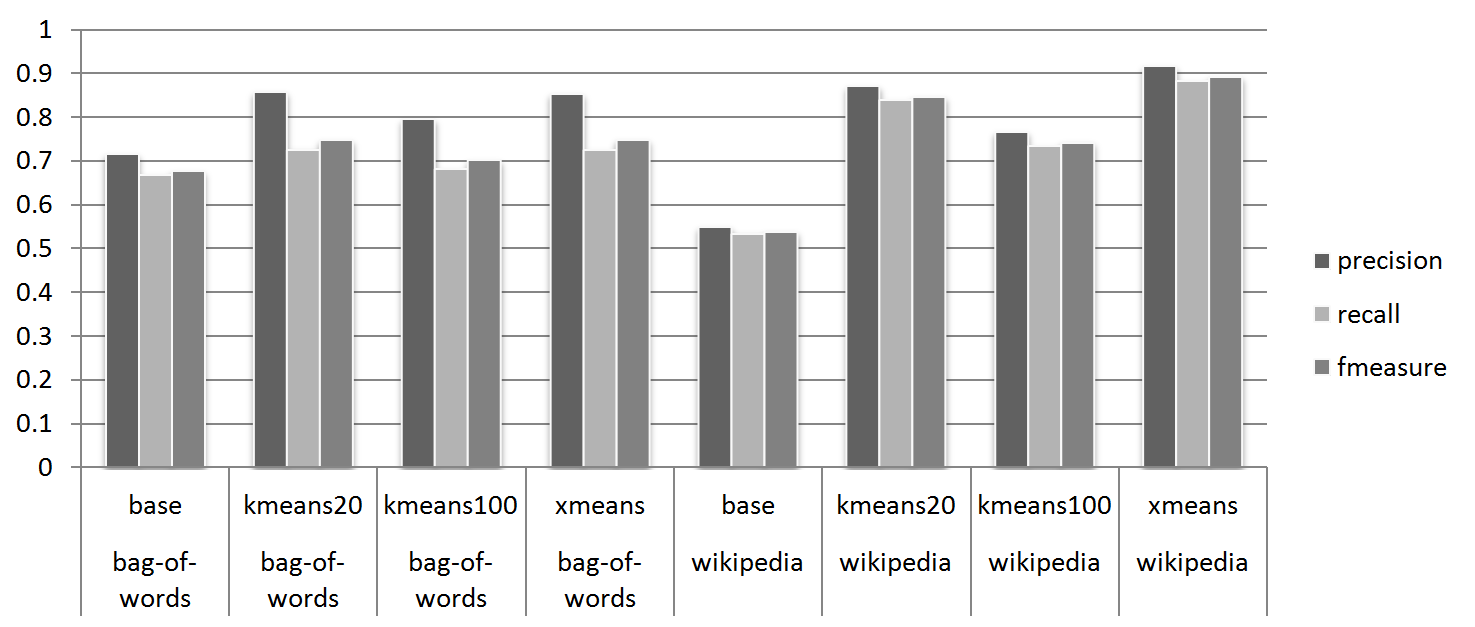
\includegraphics[width=0.7\textwidth]{svm}
    \caption{Метод опорных векторов}
\end{figure}

Данный метод (support vector machines) применим для двух классов. Основной идеей метода является попытка разделения исходной выборки с помощью гиперплоскости. В случае линейно разделимой выборки, методом ищется гиперплоскость с максимальным ``зазором'' --- суммой расстояний от плоскости до ближайших представителей обоих классов. В случае отсутствия линейной разделимости вводится понятие штрафа ($C$).
Результатом работы алгоритма является линейный классификатор задаваемый двумя параметрами: вектором $\mathbf{w}$ и константой $\mathbf{b}$. Сам алгоритм классификации задается следующим образом: $\mathrm{classify}(\mathbf{x}) = \mathrm{sign}(\mathbf{w}\cdot\mathbf{x} - b)$, где $\cdot$ --- скалярное произведение.

Стоит отметить, что в некоторых случаях применяют метод опорных векторов с каким-либо ядром. Главной идеей этого метода является замена скалярного произведения во всех операциях на какую-либо нелинейную функцию, называемую ядром. При использовании ядра, выборки, неразделимые линейным ядром, могут стать разделимыми. Однако в данной работе все случаи ядер, отличных от линейного, не рассматриваются. В частности в работе \cite{Gabrilovich:2004:TCM:1015330.1015388} сделан вывод, что для классификации текстов лучше всего подходит линейное ядро.

Для классификации более чем на два класса используется техника один-против-одного (one-against-one). Для каждой пары классов строится разделяющая гиперплоскость, в качестве итогового класса для документа выбирается тот, за который проголосовало большее число классификаторов.

\subsubsection{Деревья решений}
К данному классу алгоритмов классификации относятся алгоритмы строящие итоговый классификатор в виде дерева.
Во внутренних вершинах построенного дерева записываются условия на классифицируемый объект, в листьях --- результат классификации. Пример того, как может выглядеть дерево решения для задачи классификации людей на выживших и не выживших во время катастрофы ``Титаника''\footnote{http://ru.wikipedia.org/wiki/Титаник}, изображен на Рис. \ref{fig:titanic}. Преимуществом деревьев решений является их интерпретируемость для человека --- результат можно наглядно отобразить и проанализировать.

\begin{figure}[h!]
  \centering
    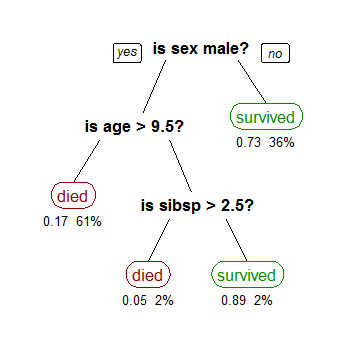
\includegraphics[width=0.7\textwidth]{titanic}
    \caption{Пример дерева принятия решений}
    \label{fig:titanic}
\end{figure}

\section{Кластеризация}
\subsection{Формальное определение}
Кластеризация --- задача машинного обучения без учителя. В данной задаче имеется множество объектов. 
Целью кластеризации является выявление групп похожих объектов, разделения объектов на классы. Главным отличием кластеризации от классификации следует считать то, что никакие характеристики групп не задаются, группы определяются полностью автоматически на основе попарной схожести объектов. 

Формально, пусть $X$ --- множество объектов, $Y$ --- множество номеров (имён, меток) кластеров. Задана функция расстояния между объектами $\rho(x,x')~$. Имеется конечная выборка объектов $X^m = \{ x_1, \dots, x_m \} \subset X$. Требуется разбить выборку на непересекающиеся подмножества, называемые ``кластерами'', так, чтобы каждый кластер состоял из объектов, близких по метрике $\rho~$, а объекты разных кластеров существенно отличались. При этом каждому объекту $x_i\in X^m$ приписывается номер кластера $y_i~$.

``Алгоритм кластеризации'' --- это функция $a\colon X\to Y$, которая любому объекту $x\in X$ ставит в соответствие номер кластера $y\in Y$. Множество $Y~$в некоторых случаях известно заранее, однако чаще ставится задача определить оптимальное число кластеров, c точки зрения того или иного ``критерия качества'' кластеризации \cite{wiki:ru-clusterization}.

Алгоритмы кластеризации, как и алгоритмы классификации, обычно имеют дело с некоторыми признаками объектов пространства $X$.

\subsection{Алгоритмы}
Входными данными для алгоритмов кластеризации выступают либо признаковые описания объектов, либо матрица попарных расстояний между объектами. Можно выделить следующие методы кластеризации: на основе графов, статистические, иерархические и на основе нейронных сетей. Стоит упомянуть, что существует задача нечеткой кластеризации, в которой, объект принадлежит кластерам с некоторой вероятностью. Далее подробней описаны алгоритмы использованные в этой работе. 

\subsubsection{Метод k-средних}
В данном алгоритме количество кластеров фиксировано величиной $k$. Задачей данного алгоритма является минимизация величины \begin{gather}
\underset{\mathbf{S}} {\operatorname{arg\,min}} \sum_{i=1}^{k} \sum_{\mathbf x_j \in S_i} \left\| \mathbf x_j - \boldsymbol\mu_i \right\|^2,
\end{gather} где $\mathbf{S}$ --- все возможные разбиения элементов $X$ на $k$ кластеров, а $\mu_i$ является центром масс кластера $S_i$. 

Задача поиска глобального минимума является NP-трудной \cite{springerlink:10.1007/s10994-009-5103-0}, однако для нее существует широко используемый алгоритм приближенного решения, находящий локальный оптимум.

Зафиксируем каким-либо образом (например случайным) $k$ первоначальных центров кластеров $m_1^{(1)}, \dots, m_k^{(1)}$. Далее алгоритм состоит из двух повторяющихся шагов:
\begin{description}
\item[Шаг присваивания] Каждому объекту из выборки $X$ сопоставляется кластер, центр которого находится к нему ближе всего: 
\begin{gather}
S_i^{(t)} = \big \{ x_p : \big \| x_p - m^{(t)}_i \big \| \le \big \| x_p - m^{(t)}_j \big \| \ \forall\ 1 \le j \le k \big\}
\end{gather}
\item[Шаг обновления] На основе объектов каждого кластера считаются новые центры: \begin{gather}
\mathbf m^{(t+1)}_i = \frac{1}{|S^{(t)}_i|} \sum_{\mathbf x_j \in S^{(t)}_i} \mathbf x_j
\end{gather}
\end{description}

Процесс заканчивается в тот момент, когда центры кластеров перестают обновляться (с какой-либо точностью). Каждый шаг алгоритма делает $O(nkt)$ действий, где $n$ --- общее количество объектов, а $t$ --- время вычисления расстояния между одной парой объектов. Данный алгоритм имеет полиномиальное количество итераций \cite{DBLP:journals/corr/abs-0904-1113}. На практике количество итераций обычно ограничивают.

\subsubsection{XMeans}
Данный алгоритм является некоторым обобщением алгоритма k-средних и использует его в своей реализации. Одним из главных отличий данного алгоритма можно назвать отсутствие требования точного количества искомых кластеров, задается лишь требуемый диапазон значений для количества кластеров. Более подробно можно прочитать в \cite{Pelleg2000}.

\section{Модель текста для классификации и кластеризации}
\label{sec:text-model}
Вышеописанные методы классификации и кластеризации применимы, если у исходных объектов есть какие-либо признаки, как это описывалось ранее. Таким образом возникает задача выделения признаков у текста.

Для решения данной задачи существует множество подходов. Опишем здесь один из самых простых. Пусть признаками в результирующем пространстве будут слова, а значениями данных признаков --- $\mathrm{tf*idf}$ данного слова относительно данного документа, где $\mathrm{tf*idf}$ определен следующим образом: \begin{gather}
\mathrm{tf}(t, d) = \frac{n_i}{\sum_k n_k} \\
\mathrm{idf}(t, D) =  \log \frac{|D|}{|d \in D : t_i \in d|} \\
\mathrm{tf*idf}(t,d,D) = \mathrm{tf}(t,d) \times \mathrm{idf}(t, D),
\end{gather} где $t$ текущее слово, $n_i$ число вхождений текущего слова в текущий документ, $\sum_k n_k$ общее количество слов в текущем документе, $d$ текущий документ, $D$ --- все документы в выборке. Величина $\mathrm{tf}$ характеризует частотность слова (терма) относительно документа, величина $\mathrm{idf}$ --- долю документов содержащих данное слово, таким образом для популярных слов величина $\mathrm{idf}$, и, соответственно $\mathrm{tf*idf}$, уменьшается.

Стоит отметить, что имеет смысл преобразовывать входной документ; к примеру, приводить слова к нормальной форме. Для данных целей служит стемминг --- процесс нахождения основы слова\footnote{http://ru.wikipedia.org/wiki/Стемминг}. Не лишено смысла применения латентно-семантического анализа\footnote{http://en.wikipedia.org/wiki/Latent\_semantic\_analysis}, для предобработки объектов. С помощью данного метода происходит выделение тематических признаков из текста. Похожий метод по выделению тематических признаков из текста с помощью метода LDA использовался в работе \cite{ramage2010characterizing}.

% другие результаты - не надо юзать ngrams
% http://know-center.tugraz.at/wp-content/uploads/2010/12/Master-Thesis-Christopher-Horn.pdf

\section{Методы оценки алгоритмов классификации}
Пусть есть построенный алгоритм классификации $a$. Для оценки качества данного алгоритма нам понадобиться дополнительная, так называемая, тестовая выборка $T$. Для данной выборки мы будем знать верные значения классов элементов. Опишем некоторые величины характеристики качества нашего алгоритма классификации: \begin{gather}
\mathrm{precision}(c) = \frac{|d \in T \colon class(d) = a(d) = c|}{|d \in T \colon a(d) = c|} \\
\mathrm{recall}(c) = \frac{|d \in T \colon class(d) = a(d) = c|}{|d \in T \colon class(d) = c|} \\
\mathrm{F}(c) = \frac{2 \mathrm{precision}(c) \mathrm{recall}(c)}{\mathrm{precision}(c) + \mathrm{recall}(c)},
\end{gather}
другими словами точность ($\mathrm{precision}$) --- это число элементов, квалифицированных правильно, по отношению к числу элементов, квалифицированных вообще, полнота ($\mathrm{recall}$) --- это число элементов, квалифицированных правильно, по отношению к общему размеру класса, а F-мера ($\mathrm{F}$) --- среднее гармоническое точности и полноты.

Недостатком этих величин является то, что они являются специфичными для классов. Введем обобщающие величины, характеризующие построенный алгоритм в целом: \begin{gather}
\mathrm{precision_{macro}} = \frac{1}{|C|} \sum_{c \in C} \mathrm{precision}(c) \\
\mathrm{recall_{macro}} = \frac{1}{|C|} \sum_{c \in C} \mathrm{recall}(c) \\
\mathrm{F_{macro}} = \frac{1}{|C|} \sum_{c \in C} \mathrm{F}(c).
\end{gather}

Данные величины можно использовать для оценки качества построенного классификатора.

\section{Методы тестирования классификаторов}
В простейшем случае нам дана как обучающая, так и тестовая выборка. Однако бывают случаи, когда тестовая выборка не дана. В этом случае разумно использовать часть обучающей выборки в качестве тестовой. 

Одним из примеров использования такого подхода является ``перекрёстная проверка'' (cross-validation). В данном методе обучающая выборка разбивается на $k$ частей, далее происходим обучение классификатора на $k-1$ части, и тестирование на оставшейся части. Процедура повторяется $k$ раз, а полученные результаты оценки качества, например, усредняются.